%!TEX root = main.tex
All code needed to reproduce examples in this section can be found at \url{https://github.com/unstable-zeros/robust-sls}. We consider a scaled doubly-stochastic chain system described by the following dynamics:
\begin{equation}\label{eq:chain}
\begin{array}{rcl}
x^1_{t+1} &=& \rho\left[(1-\alpha)x^1_t + \alpha x^2_t\right] + u^1_t\\
x^i_{t+1} &=& \rho\left[\alpha x^{i-1}_t + (1-2\alpha)x^i_t + \alpha x^{i+1}_t\right] + u^i_t,\\
&& \text{ for $i=2,\dots,N-1$,} \\
 x^N_{t+1} &=& \rho\left[\alpha x^{N-1}_t + (1-\alpha)x^N_t\right] + u^N_t
 \end{array}
\end{equation}
where the $x^i_t, u^i_t \in \R$ are the scalar state and inputs, respectively, of the subsystems, and we set the number of scalar subsystems $N=50$, the scaling factor $\rho = 0.5$, and the coupling constant $\alpha = 0.49$.  

We solve the robust performance performance problem \eqref{eq:constraints} under both centralized and localized distributed constraints with a norm bound on the uncertainty of $\epsilon = 0.55$, and cost matrices $C^\top = [I_N, 0^\top]^\top$ \& $D^\top = [0^\top, 5I_N]$.  For both settings, we impose an FIR horizon of $T=10$ when solving the robust performance problem \eqref{eq:constraints}.  Additionally, we enforce that the corresponding system responses satisfy $d$-locality constraints -- intuitively, these constraints ensure that in closed loop, the disturbance striking node $i$ only affects nodes $j$ satisfying $|j-i|\leq d$.\footnote{In the interest of clarity, we do not enforce communication delay constraints, but note that both communication delay and locality constraints can be enforced through suitable sparsity constraints on the system response variables: see \cite{anderson2019system} for details.}

By bisecting on $\gamma$, we determine that the optimal robust performance level is $\gamma = 5.57$ for both centralized and distributed controllers, where for the distributed localized controller we set the locality diameter to $d=2$.  That there is no gap between centralized and distributed is not surprising because: (i) we impose no communication delay constraints, and (ii) $\mathcal{L}_1$ optimal control leads to deadbeat optimal closed loop responses, which will consequently also be (approximately) localized in space as well.  We note that the nominal $\mathcal{L}_1$ norms of the closed loop systems for the centralized and distributed localized controllers are both $2.5$.  Comparing these to the norms achieved by the optimal $\mathcal{L}_1$ controllers (i.e., those computed by minimizing the performance cost with $\epsilon = 0$) of $1.43$ and $2.47$, respectively, we see that while there is an appreciable degradation in nominal performance in the centralized setting, there is nearly no degradation in the localized distributed setting!  We conjecture that this is due to the sparsity of the augmented plant $\tf M$ defined by the system response $\Phih$, which constrains both robust and nominal systems to behave similarly.

To empirically test this conjecture, we examine the evolution of the closed loop norm of the nominal and robust controllers to perturbations of the form $\DA = \mathrm{blkdiag}(\kappa I, \kappa I, \dots)$ and $\DB = 0$, for $\kappa \in [0,\epsilon]$, for varying locality parameters $d\in\{2,5,10\}$, where $d=10$ corresponds to the centralized setting.  The results are displayed in Fig \ref{fig:kappa}.  We show only the results for $d=2$ and $d=5$, as the result for $d=5$ and $d=10$ are indistinguishable -- as can be observed, in the ``extremely'' localized setting of $d=2$, the degrees of freedom are limited such that robust and nominal control behave similarly; in contrast, when $d=5$, the robust controller enjoys improved performance for larger values of $\kappa$, at the expense of degraded performance at lower values.  Our approach therefore allows for a principled exploration of tradeoffs between synthesis/implementation complexity (as measured by $d$), nominal performance, and robust performance for large-scale distributed systems.

\begin{figure}
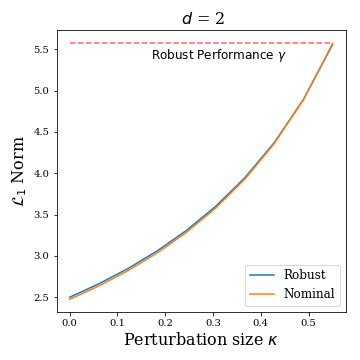
\includegraphics[width=.45\columnwidth]{d2.png}~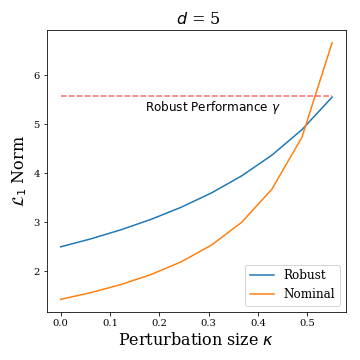
\includegraphics[width=.45\columnwidth]{d5.png}
\caption{Performance of a robust controller and a nominally optimal controller for for two decentralized chains, with disturbances  $\DA = \mathrm{blkdiag}(\kappa I, \kappa I, \dots)$. As $\kappa$ increases to $\epsilon = 0.55$, performance of the robust controller meets the robust performance bound $\gamma$ \eqref{eq:constraints}.}
\label{fig:kappa}
\end{figure}

%Finally we note that even without exploiting any of the underlying partial separability of the resulting problem (see \cite{wang2018separable}), we are able to solve the resulting centralized and distributed localized feasibility problems \eqref{eq:constraints} in 29s and 114s,\footnote{The majority of this time was spent on pre-processing by MOSEK: the actual solve time required by the optimizer was under 1s.} respectively, on a 2.3GHz 8 Core MacBook Pro with 32 GB of RAM using CVXPY \cite{diamond2016cvxpy} and MOSEK \cite{andersen2000mosek}.